\documentclass[final]{beamer}
\mode<presentation> {
	\usetheme{wtsi}
}
\usepackage[english]{babel}
\usepackage[latin1]{inputenc}
\usepackage{amsmath,amsthm, amssymb, latexsym}
\usepackage{tikz}
\usetikzlibrary{shapes.geometric, arrows}
\usepackage[orientation=portrait,size=a0,scale=1.4,debug]{beamerposter}
\usefonttheme[onlymath]{serif}
\boldmath
 
\title{Using haploid human DNA to design and evaluate the HiSeq X data processing strategy}
\author{Martin O. Pollard, Thomas M. Keene, Shane A. McCarthy, Joshua C. Randall, Richard M. Durbin}
\date{Today}

\begin{document}
\begin{frame}
    \begin{columns}
    % ---------------------------------------------------------%
    % Set up a column 
    \begin{column}{.49\textwidth}
        \begin{beamercolorbox}[center,wd=\textwidth]{postercolumn}
            \begin{minipage}[T]{.95\textwidth}  % tweaks the width, makes a new \textwidth
            \parbox[t][\columnheight]{\textwidth}{
            \begin{block}{Introduction}
            The Illumina HiSeq X promises a reduction in sequencing cost but has required changes to the chemistry, software, and output.  To take advantage of this we have designed experiments using well characterised samples to explore what we need to do to best take advantage of these improvements. 
            \end{block}
            \begin{block}{Method}
                \tikzstyle{io} = [trapezium, trapezium left angle=70, trapezium right angle=110, minimum width=3cm, minimum height=1cm, text centered, draw=black, fill=blue!30]
                \tikzstyle{process} = [rectangle, minimum width=9cm, minimum height=3cm, text centered, draw=black, fill=orange!30]
                \tikzstyle{decision} = [diamond, minimum width=9cm, minimum height=3cm, text centered, draw=black, fill=green!30]
                \tikzstyle{arrow} = [thick,->,>=stealth]
                \centering
                \begin{tikzpicture}[node distance=4.5cm]
                    \node (in1) [io] {Illumina RTA};
                    \node (pro1) [process, below of=in1] {Mapper};
                    \node (pro2) [process, below of=pro1] {Fix Mate Pairing};
                    \node (pro3) [process, below of=pro2] {Sort};
                    \node (pro4) [process, below of=pro3] {Mark Duplicates};
                    \node (pro5) [process, below of=pro4] {Call};
                    \node (dec1) [decision, below of=pro5, yshift=-1.5cm] {Evaluate};
                    \draw [arrow] (in1) -- (pro1);
                    \draw [arrow] (pro1) -- (pro2);
                    \draw [arrow] (pro2) -- (pro3);
                    \draw [arrow] (pro3) -- (pro4);
                    \draw [arrow] (pro4) -- (pro5);
                    \draw [arrow] (pro5) -- (dec1);
                \end{tikzpicture}
            \end{block}
            \begin{block}{Results}
            \end{block}
            \vfill
                      }
          % ---------------------------------------------------------%
          % end the column

            \end{minipage}
        \end{beamercolorbox}
    \end{column}
        \begin{column}{.49\textwidth}
        \begin{beamercolorbox}[center,wd=\textwidth]{postercolumn}
            \begin{minipage}[T]{.95\textwidth}  % tweaks the width, makes a new \textwidth
            \parbox[t][\columnheight]{\textwidth}{
            \begin{block}{}
                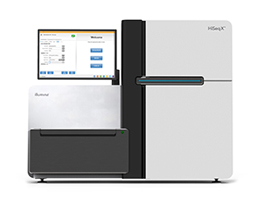
\includegraphics[width=.95\linewidth]{images/hiseq-x}
            \end{block}
            \begin{block}{What has changed?}
                \begin{itemize}
                    \item Error Profile (particularly context specific errors).
                    \item Quality Score Binning by default.
                    \item Read length increased to 150bp.
                    \item New Mappers available and required to take advantage of read length.
                \end{itemize}
            \end{block}
            \begin{block}{Conclusion}
                Lots and lots of DATA!
            \end{block}
            \begin{block}{Acknowledgements}
                Sanger Core Sequencing Team for providing the data. Sanger NPG for quality control.
            \end{block}
            \vfill
                      }
          % ---------------------------------------------------------%
          % end the column

            \end{minipage}
        \end{beamercolorbox}
    \end{column}
    \end{columns}
\end{frame}
\end{document}

